\documentclass[12pt,a4paper]{article}
\usepackage[spanish,es-tabla]{babel}
\usepackage[utf8]{inputenc}
\usepackage{graphicx}
\usepackage{hyperref}
\usepackage{makecell}
\usepackage{float}
\usepackage{natbib}

\title{Proyecto}
\author{Gabriel Abellán Rodríguez}
\date{\today}

\begin{document}
\begin{titlepage}
    \centering
    
\includegraphics[width=0.4\textwidth]{images/LogoRiberaNuevo.png}\par
    \vspace{1cm}
    {\bfseries\LARGE I.E.S. Ribera del Tajo \par}
    \vspace{1cm}
    {\scshape\Large Técnico Superior en Administración de Sistemas Informáticos en Red
    \par}
    \vspace{3cm}
    {\scshape\Huge Tarea PIMAS 02 \par}
    \vspace{3cm}
    {\itshape\Large Proyecto intermodular de Administración de Sistemas Informáticos en Red \par}
    \vfill
    {\Large Autor:\par}
    {\Large Gabriel Abellán Rodríguez \par}
    \vfill
    {\Large \today \par}
\end{titlepage}

\tableofcontents
\newpage

\section{Introducción}

El presente proyecto tiene como objetivo fundamental el diseño, desarrollo e implementación de una plataforma web transaccional orientada a la comercialización e información de juegos de cartas coleccionables (JCC). Este sector ha experimentado un crecimiento sostenido en los últimos ejercicios, tanto en volumen de usuarios como en el consumo de productos asociados. La solución propuesta no solo constituye un entorno de comercio electrónico B2C (Business-to-Consumer) para la adquisición de productos y accesorios, sino que también actúa como un repositorio documental y formativo para usuarios de diversos niveles de experiencia.

La plataforma se estructura en módulos funcionales diferenciados: una tienda en línea para la comercialización de productos, un apartado de guías técnicas introductorias para los principales sistemas de juego del mercado, y una sección de divulgación normativa. Este enfoque centraliza servicios y conocimientos que habitualmente se encuentran fragmentados en la red.

A nivel de interfaz de usuario (UI) y experiencia de usuario (UX), el diseño se basa en principios de accesibilidad, usabilidad y diseño adaptativo (Responsive Web Design), garantizando la correcta visualización en dispositivos de escritorio y móviles. Adicionalmente, se ha implementado soporte multi-idioma (español e inglés) para facilitar la internacionalización del servicio.

El desarrollo de esta infraestructura tecnológica constituye la aplicación práctica de los conocimientos adquiridos durante el ciclo formativo de grado superior en Administración de Sistemas Informáticos en Red (ASIR). Esto abarca desde el despliegue de la capa de presentación (frontend) y lógica de negocio (backend), hasta el diseño de la persistencia de datos, la configuración de topologías de red seguras y el establecimiento de políticas de alta disponibilidad.

\newpage
\section{Módulos Implicados}
\label{Modulos}

El desarrollo arquitectónico e implementación técnica del proyecto se fundamentan en las siguientes áreas de conocimiento:

\begin{itemize}
    \item \textbf{Administración de Sistemas Operativos:} Despliegue y configuración de entornos de servidor (Windows Server y distribuciones GNU/Linux). Implementación de rutinas de automatización (scripts Bash) para la gestión de copias de seguridad de la base de datos (Disaster Recovery).
    \item \textbf{Planificación y Administración de Redes:} Diseño de la topología lógica, segmentación mediante VLANs y configuración de reglas de enrutamiento y cortafuegos para aislar entornos críticos.
    \item \textbf{Fundamentos de Hardware:} Planificación de los requisitos físicos para la infraestructura de servidores y sistemas de almacenamiento necesarios para garantizar el rendimiento operativo.
    \item \textbf{Inglés:} Integración de funcionalidades de internacionalización en la plataforma, permitiendo la conmutación dinámica del contenido entre español e inglés.
    \item \textbf{Lenguaje de Marcas y Sistemas de Gestión de Información:} Construcción de la capa de presentación mediante HTML5 y CSS3, aplicando metodologías de diseño modular. Integración de interactividad asíncrona mediante JavaScript (peticiones Fetch y notificaciones tipo toast).
    \item \textbf{Implantación de Aplicaciones Web:} Configuración de servidores web (Apache/Nginx) y despliegue del entorno de ejecución PHP para la lógica de negocio.
    \item \textbf{Gestión de Bases de Datos:} Diseño e implementación del esquema relacional en motores MySQL/MariaDB. Uso de procedimientos almacenados y disparadores (Triggers) para garantizar la integridad referencial y automatizar procesos internos.
    \item \textbf{Seguridad y Alta Disponibilidad:} Aplicación de políticas de bastionado (Hardening), cifrado asimétrico para accesos (SSH), configuración de túneles seguros (TLS/SSL) y diseño de infraestructuras redundantes.
    \item \textbf{Itinerario Personal para la Empleabilidad:} Formulación del plan de Prevención de Riesgos Laborales (PRL) asociado al entorno tecnológico y logístico del proyecto.
\end{itemize}

\newpage
\section{Estudio de Mercado y Viabilidad Comercial}
\label{EstudioMercado}

\textbf{Público Objetivo:} El segmento de mercado principal comprende usuarios de entre 15 y 35 años, con perfiles orientados al coleccionismo y al juego competitivo de la franquicia Pokémon. La fase inicial de despliegue logístico se acotará al territorio nacional (España), con proyecciones de escalabilidad hacia el mercado europeo (Cross-border e-commerce) a medio plazo.

\textbf{Análisis de la Competencia:} El ecosistema de venta de JCC presenta una alta saturación. Para establecer una ventaja competitiva, la plataforma propuesta enfatiza una experiencia de usuario (UX) superior y tiempos de respuesta logísticos optimizados. Entre los principales actores del mercado se identifican:
    
    \begin{itemize}
        \item \textbf{Canales Oficiales (Pokémon Center):} Presentan alta fiabilidad, pero adolecen de precios premium y frecuentes roturas de stock.
        \item \textbf{Plataformas Marketplace (Cardmarket):} Ofrecen gran volumen, pero la naturaleza descentralizada incrementa los riesgos de fraude y encarece los costes logísticos (múltiples envíos).
        \item \textbf{Retail Local:} Disponen de proximidad, pero generalmente aplican márgenes comerciales elevados que restan competitividad frente a soluciones digitales puras.
    \end{itemize}

\textbf{Demanda:} El mercado de coleccionables mantiene una curva de demanda sostenida y alcista, caracterizada por su resiliencia incluso en periodos de contracción económica, impulsada por la nostalgia y el factor especulativo de los activos (cartas).

\textbf{Estrategia de Penetración (Marketing):} Se priorizará el marketing de contenidos en plataformas de alta tasa de retención (Instagram, YouTube Shorts) para canalizar tráfico orgánico. Simultáneamente, se aplicarán técnicas de optimización en motores de búsqueda (SEO) y marcado semántico para mejorar la indexabilidad de la plataforma.

\section{Análisis DAFO (Debilidades, Amenazas, Fortalezas y Oportunidades)}
\label{DAFO}

\textbf{Debilidades:}
\begin{itemize}
    \item Dependencia inicial en la gestión manual de operaciones logísticas, control de inventarios y atención de incidencias.
    \item Posicionamiento nulo en la fase de lanzamiento (Start-up), requiriendo un esfuerzo intensivo para capturar cuota de mercado frente a competidores consolidados.
    \item Alta dependencia del flujo de lanzamientos (novedades) dictado por el fabricante.
    \item Requerimiento de capital de trabajo (Working Capital) elevado para el acopio inicial de inventario con márgenes competitivos.
\end{itemize}

\textbf{Amenazas:}
\begin{itemize}
    \item Roturas de cadena de suministro por parte de los distribuidores mayoristas, que podrían interrumpir el flujo de ventas.
    \item Riesgo operativo derivado de la introducción de falsificaciones ("proxies") de alta fidelidad en el mercado secundario de compraventa.
    \item Fluctuaciones en las tarifas de los operadores logísticos (e.g., Correos, SEUR), que pueden impactar negativamente en el margen de beneficio neto.
\end{itemize}

\textbf{Fortalezas:}
\begin{itemize}
    \item Producto de alta demanda y liquidez, con una base de consumidores altamente fidelizada y dispuesta a la compra recurrente.
    \item Estructura de costes operativos fijos iniciales mínimos (Bootstrapping), al centralizar las operaciones en un entorno logístico propio y prescindir temporalmente de locales comerciales.
    \item Arquitectura web de grado empresarial (Premium UI/UX, integración de IA, notificaciones asíncronas), que transmite confiabilidad y modernidad frente a plataformas heredadas (Legacy).
\end{itemize}

\textbf{Oportunidades:}
\begin{itemize}
    \item Expansión continua del mercado de coleccionables en el ecosistema digital europeo.
    \item Posibilidad de generar sinergias mediante la creación de contenido viral en redes sociales para reducir los costes de adquisición de clientes (CAC).
    \item Escalabilidad horizontal del catálogo hacia productos adyacentes de alto margen (accesorios de protección, álbumes, merchandising).
\end{itemize}

\newpage
\section{Catálogo de Servicios Digitales}
\label{Servicios}

La arquitectura del servicio ha sido diseñada para minimizar la fricción en el proceso de conversión (compra) y proporcionar valor añadido mediante soluciones tecnológicas avanzadas.

\subsection{Comercio Electrónico B2C}
El servicio central consiste en una plataforma de e-commerce transaccional. La base de datos segmenta el catálogo en dos líneas principales: productos sellados (cajas, sobres) y el mercado secundario de activos individuales (cartas sueltas).

\subsection{Gestión Logística}
Se ha implementado un flujo de gestión de pedidos integrado, diseñado para coordinar la expedición a través de operadores logísticos nacionales, garantizando el acondicionamiento protector ("packaging" especializado) para prevenir la depreciación del activo durante el tránsito.

\subsection{Atención al Cliente mediante Inteligencia Artificial}
Para optimizar los recursos de soporte, se han integrado servicios basados en Inteligencia Artificial mediante consumo de APIs RESTful:
\begin{itemize}
    \item \textbf{PimasBot AI:} Asistente virtual impulsado por los modelos fundacionales de Google Gemini, capaz de procesar lenguaje natural (NLP) para resolver consultas operativas de Nivel 1.
    \item \textbf{PokeLens (Computer Vision):} Módulo de reconocimiento de imágenes que, apoyándose en la IA de visión computacional, clasifica y detecta automáticamente tarjetas subidas por el usuario, automatizando la búsqueda en el catálogo.
\end{itemize}

\subsection{Autenticación y Verificación de Identidad}
Se ha implementado un flujo de autenticación robusto. La plataforma requiere la validación de cuentas mediante el envío de códigos de un solo uso (OTP) a través de un servidor de correo saliente (SMTP). Este mecanismo previene el alta de cuentas sintéticas y garantiza la trazabilidad de los usuarios.

\subsection{Políticas de Restricción y Calidad de Servicio (QoS)}
Para garantizar la disponibilidad de la plataforma y mitigar riesgos de seguridad (como ataques de denegación de servicio a nivel de aplicación - Capa 7 OSI), se aplican principios de acceso condicional. Funcionalidades de alto consumo computacional o integraciones con APIs externas (Carrito de compra, llamadas a Gemini AI) están restringidas exclusivamente a sesiones autenticadas. Esta política de "Rate Limiting" implícita previene la saturación de CPU/RAM y el agotamiento de cuotas de facturación de servicios de terceros por parte de agentes automatizados (Bots).

\subsection{Diseño de Interfaz Asíncrono}
La experiencia de usuario se ha optimizado mediante el uso de JavaScript asíncrono (AJAX/Fetch) y CSS3 avanzado. Las interacciones con la base de datos (e.g., adición de ítems al carrito) no requieren la recarga del documento (Document Object Model), operando en segundo plano e informando al usuario mediante componentes visuales no intrusivos ("Toast Notifications") y micro-animaciones.

\newpage
\section{Arquitectura de Persistencia de Datos}
La persistencia de información se soporta sobre un motor de bases de datos relacional (MySQL/MariaDB). En la fase de desarrollo se ha optado por entornos de prueba locales, con un plan de migración hacia instancias contenerizadas para la fase de producción, garantizando así la inmutabilidad del entorno y eliminando dependencias tipo XAMPP.

\subsection{Esquema Relacional}
El modelo de datos garantiza la integridad referencial y se apoya en restricciones (Constraints) y disparadores lógicos (Triggers) para automatizar el control de concurrencia y los flujos de inventario.

\begin{figure}[H]
    \centering
    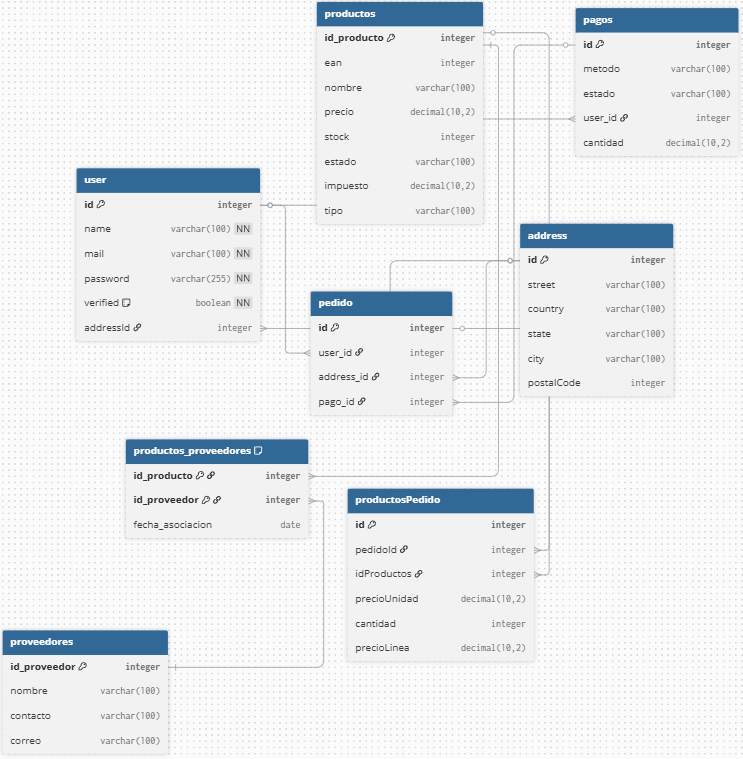
\includegraphics[width=0.8\linewidth]{images/dbdiagram.png}
    \caption{Diagrama Entidad-Relación de la base de datos.}
\end{figure}

\newpage
\section{Stack Tecnológico y Desarrollo Web}
\label{PaginaWeb}

La solución adopta una arquitectura cliente-servidor clásica, segmentada en las capas de presentación, lógica de negocio y persistencia.

\subsection{Definición del Stack}
\begin{itemize}
    \item \textbf{Capa de Presentación (Frontend):} Desarrollada en HTML5 semántico y CSS3 puro para garantizar un renderizado ligero y de alto rendimiento (Zero-dependency architecture). Se integra JavaScript nativo (Vanilla JS) para gestionar el estado de la interfaz y las llamadas asíncronas.
    \item \textbf{Capa Lógica (Backend):} Procesamiento soportado por PHP, gestionando el control de sesiones seguras, la validación de entrada (Input sanitization) contra ataques de inyección SQL (SQLi) y Cross-Site Scripting (XSS). La gestión de contraseñas se implementa mediante funciones de derivación de claves criptográficas (BCRYPT).
    \item \textbf{Capa de Datos (SQL):} Desplegada sobre MySQL/MariaDB, utilizando sentencias preparadas (Prepared Statements) en PHP (PDO/MySQLi) para garantizar la seguridad transaccional.
    \item \textbf{Integración de Servicios de Terceros (APIs):} Conexiones asíncronas hacia infraestructuras Cloud (Google Gemini) para dotar a la plataforma de capacidades de inteligencia artificial generativa y visión computacional.
\end{itemize}

\subsection{Diseño Adaptativo (Responsive Design)}
El marco de estilos (CSS) se ha estructurado mediante la metodología de separación de responsabilidades (archivos independientes para tipografías, componentes, disposición espacial). Mediante el uso de consultas de medios ("Media Queries"), la interfaz se adapta fluidamente a distintas resoluciones, garantizando la operatividad (Mobile-First approach).

\newpage
\section{Continuidad de Negocio: Backup y Recuperación (Disaster Recovery)}
\label{Backup}

La integridad y disponibilidad de la información son críticas. Se han establecido políticas de redundancia para prevenir la pérdida de datos ante fallos de hardware, errores humanos o compromisos de seguridad.

La estrategia de respaldos se automatiza a nivel de sistema operativo mediante tareas programadas (Cron jobs en Linux) y scripts Bash, encargados de ejecutar volcados (Dumps) de la base de datos a intervalos regulares. Estos archivos resultantes son comprimidos y almacenados en repositorios aislados de la red pública, posibilitando una restauración rápida (RTO/RPO optimizados) en caso de contingencia.

\newpage

\section{Estudio de Viabilidad Técnica y Económica}
\label{PlanNegocio}

\subsection{Modelo de Ingresos (Revenue Model)}
La viabilidad financiera del proyecto se estructura en tres verticales de negocio:

\begin{enumerate}
    \item \textbf{Retail Tradicional (Producto Sellado):} Adquisición de inventario a distribuidores mayoristas (B2B) y comercialización a precio de venta recomendado (PVR), asegurando márgenes operativos predecibles.
    \item \textbf{Mercado Secundario (Cartas Sueltas):} Constituye el núcleo de rentabilidad, basado en el arbitraje y la tasación experta del estado de los activos ("Grading"). Los márgenes brutos en esta vertical pueden alcanzar o superar el 50\%.
    \item \textbf{Cross-Selling (Accesorios):} Comercialización de periféricos de protección y almacenamiento (fundas, carpetas). Estos productos actúan como complementos indispensables para el cliente, incrementando significativamente el valor medio del ticket de compra.
\end{enumerate}

\subsection{Estructura Jurídico-Fiscal}
Para la fase de lanzamiento (Seed stage), la estructura jurídica más eficiente es el alta en el Régimen Especial de Trabajadores Autónomos (RETA). Esta figura minimiza las barreras de entrada burocráticas y evita la exigencia de inmovilización de capital social (como requeriría una S.L.), permitiendo la facturación legal, la liquidación del IVA y la deducción del Impuesto sobre Sociedades/IRPF aplicable a los gastos de infraestructura IT y aprovisionamiento.

\subsection{Plan de Inversiones (CAPEX)}
La estimación del gasto de capital inicial (Capital Expenditure) necesario para el despliegue técnico y logístico se detalla a continuación:

\begin{table}[H]
    \centering
    \begin{tabular}{|l|r|}
        \hline
        \textbf{Concepto de Inversión Inicial} & \textbf{Coste Estimado} \\
        \hline
        Hardware de Red y Computación (Servidor, Switch L2/L3, Router) & 1.300 € \\
        \hline
        Licenciamiento de Software (Windows Server u otros) & 600 € \\
        \hline
        Infraestructura Cloud (Dominio y VPS Anual) & 80 € \\
        \hline
        Aprovisionamiento de Inventario Inicial & 2.500 € \\
        \hline
        Material Logístico y Embalaje & 150 € \\
        \hline
        \textbf{Total Inversión Inicial (CAPEX)} & \textbf{4.630 €} \\
        \hline
    \end{tabular}
    \caption{Previsión de inversión de capital inicial (CAPEX).}
\end{table}

El retorno de la inversión (ROI) se estima en un plazo de 18 meses. La asunción interna de las labores de administración de sistemas e ingeniería de software (In-house development) reduce drásticamente los gastos operativos (OPEX) asociados a la externalización.

\subsection{Escalabilidad Operativa}
El modelo de negocio nace bajo el concepto de Bootstrapping, centralizando temporalmente la logística y el alojamiento de los servidores perimetrales en instalaciones residenciales adaptadas para eliminar costes fijos de arrendamiento comercial.

No obstante, la infraestructura técnica y el modelo de negocio están diseñados para el escalado operativo. Ante el aumento sostenido del tráfico transaccional, se contemplan las siguientes fases de expansión:
\begin{enumerate}
    \item Migración logística hacia naves industriales o centros de distribución urbanos (Hubs).
    \item Contratación de personal operativo para el cumplimiento de pedidos (Fulfillment).
    \item Transición de la infraestructura local a gabinetes enrackables estándar industriales (Rack 19") o migración completa hacia servicios IaaS (Infrastructure as a Service) en proveedores Cloud, asegurando ancho de banda simétrico garantizado.
\end{enumerate}

\section{Cumplimiento Normativo y Privacidad (RGPD/LOPD)}
\label{LOPD}

El diseño de la plataforma se fundamenta en el principio de "Privacidad por Diseño", garantizando el estricto cumplimiento del Reglamento General de Protección de Datos (RGPD) europeo y la normativa nacional equivalente.

\begin{itemize}
    \item \textbf{Consentimiento Informado:} La arquitectura de registro incorpora validaciones explícitas ("Opt-in") donde el usuario autoriza el tratamiento de sus datos de carácter personal, circunscritos exclusivamente a la finalidad logística y fiscal del servicio.
    \item \textbf{Cifrado en Reposo (Data at Rest):} Bajo ningún concepto las credenciales de acceso se almacenan en texto plano. Las contraseñas son sometidas a derivación criptográfica mediante el algoritmo BCRYPT (con factor de coste adaptativo) antes de su inserción en la base de datos.
    \item \textbf{Protección contra Autenticación Automatizada:} Se han desplegado políticas de limitación de tasa (Rate Limiting) a nivel de la base de datos y aplicación para mitigar ataques de fuerza bruta o relleno de credenciales (Credential Stuffing). Tres fallos consecutivos en el proceso de autenticación desencadenan un bloqueo temporal de la cuenta ("Lockout" de 15 minutos).
    \item \textbf{Política de Rastreo (Cookies):} La plataforma minimiza la recopilación de telemetría. Se emplean exclusivamente cookies técnicas o de sesión, estrictamente necesarias para el mantenimiento del estado transaccional (autenticación y carrito de compra), sin utilizar rastreadores de terceros para perfiles publicitarios.
\end{itemize}

\newpage
\section{Prevención de Riesgos Laborales (PRL) en Entornos IT}
\label{PRL}

Atendiendo a la naturaleza de las operaciones técnicas y logísticas, se establecen los siguientes protocolos preventivos:

\begin{itemize}
    \item \textbf{Ergonomía y Riesgos Psicosociales (PVD):} Para mitigar la fatiga visual y musculoesquelética derivada del uso prolongado de Pantallas de Visualización de Datos, se prescribe el uso de mobiliario ergonómico certificado, pautas de descanso visual (Regla 20-20-20) e iluminación perimetral antideslumbrante en los puestos de ingeniería.
    \item \textbf{Higiene Postural en Logística:} La manipulación manual de cargas (recepción de inventario y expedición) se regirá por protocolos biomecánicos de levantamiento, manteniendo la verticalidad espinal para prevenir hernias o distensiones lumbares.
    \item \textbf{Seguridad Eléctrica en CPD (Centro de Proceso de Datos):} El mantenimiento preventivo y correctivo del hardware de red y servidores exigirá protocolos antiestáticos (descarga a tierra, pulseras ESD), retirada de elementos metálicos personales y la manipulación de fuentes de alimentación bajo condiciones de aislamiento térmico y eléctrico.
\end{itemize}

\newpage
\section{Sistemas Operativos y Directorios Corporativos}
\label{SistemasOperativos}

La arquitectura prescinde de entornos monolíticos de desarrollo (como XAMPP), apostando por infraestructuras distribuidas y robustas. Se emplean entornos Microsoft Windows Server para alojar la lógica de negocio en producción (IIS) y distribuciones GNU/Linux para asegurar la persistencia de datos y el balanceo de carga perimetral.

\section{Bastionado de Servidores (Hardening) y Ciberseguridad Activa}
\label{Hardening}

Con anterioridad a la exposición pública de los servicios, los nodos anfitriones son sometidos a procesos rigurosos de "Hardening" operativo. El objetivo es reducir drásticamente la superficie de ataque explotable de los demonios subyacentes.

\subsection{Aseguramiento de los Protocolos de Administración (SSH)}
El servicio de administración remota OpenSSH se configura mediante alteraciones restrictivas en sus archivos de configuración subyacentes (\texttt{/etc/ssh/sshd\_config}):

\begin{enumerate}
    \item \textbf{Inhabilitación de Autenticación Clásica y Escalada Root:} Prohibición absoluta de accesos remotos basados en contraseña (\texttt{PasswordAuthentication no}) y revocación de los permisos de acceso de red directos para el superusuario (\texttt{PermitRootLogin no}).
    \item \textbf{Criptografía Asimétrica Obligatoria (Claves RSA/ED25519):} La autenticación requiere la presentación y correspondencia de pares de claves criptográficas de alta densidad provistas por el administrador, neutralizando la viabilidad de cualquier ataque de fuerza bruta o diccionario matemático.
    \item \textbf{Protección Dinámica contra Intrusiones (Fail2Ban/IPS):} Despliegue del motor reactivo Fail2Ban para la auditoría de registros del sistema (Syslog/Auth.log). Ante patrones iterativos de intentos fallidos provenientes de una IP externa, el sistema interactúa de forma automatizada con el cortafuegos interno (Netfilter/IPtables) para aislar (Baneo) el nodo hostil en tiempo real.
\end{enumerate}

\subsection{Criptografía en Tránsito (TLS/SSL y Let's Encrypt)}
La confidencialidad de la información transaccionada entre la capa de presentación y el cliente exige la obliteración del protocolo de texto plano (HTTP). Se ha establecido el cifrado integral de la comunicación:

\begin{itemize}
    \item \textbf{Certificación Automatizada:} Implementación del protocolo ACME mediante el cliente Certbot para la expedición, renovación desatendida y firma de certificados digitales validados por la Autoridad de Certificación Let's Encrypt.
    \item \textbf{Redirección Forzosa (HSTS):} El balanceador de carga y los servidores web imponen políticas estrictas de redirección permanente (HTTP 301) forzando el transporte de datos exclusivamente a través del puerto seguro HTTPS (TCP 443), previniendo vulnerabilidades de degradación de protocolo y secuestros de sesión (Man In The Middle - MITM).
\end{itemize}

\subsection{Cortafuegos de Nivel de Host (UFW / IPtables)}
Con independencia del cortafuegos perimetral (pfSense), cada nodo anfitrión incluye una política de denegación predeterminada ("Deny-All / Drop by Default") en su cortafuegos lógico (Uncomplicated Firewall - UFW). Exclusivamente se autoriza la apertura (Allow In) de puertos esenciales: el servicio SSH ofuscado y el puerto de escucha del contenedor inverso, cerrando de forma absoluta el acceso directo a los restantes 65.535 puertos lógicos.

\section{Infraestructura y Segmentación de Red}
\label{sec:Infraestructura}
El diseño de la topología de red constituye el núcleo crítico del despliegue. La arquitectura se fundamenta en principios de defensa en profundidad y segmentación lógica para aislar los entornos de producción y mitigar posibles brechas de seguridad.

\subsection{Enrutamiento y Segmentación Perimetral (pfSense)}
La red corporativa se administra mediante un cortafuegos y enrutador pfSense, dividiendo la infraestructura en tres zonas de seguridad estancas:
\begin{itemize}
    \item \textbf{Zona WAN:} Interfaz de salida a Internet y puerta de enlace exterior.
    \item \textbf{Zona Desmilitarizada (DMZ - 192.168.10.0/24):} Red perimetral expuesta controladamente. Aloja el balanceador de carga HAProxy y los servidores web frontales. Es la única zona que procesa tráfico proveniente del exterior (puertos HTTP/HTTPS).
    \item \textbf{Red Interna Protegida (LAN - 192.168.20.0/24):} Segmento hermético donde reside el clúster de bases de datos MariaDB y el servidor de monitorización Zabbix. Esta zona no tiene exposición directa a Internet, y solo admite conexiones específicas y auditadas desde la DMZ (como el tráfico TCP por el puerto 3306).
\end{itemize}

\section{Memoria Técnica: Alta Disponibilidad (HA)}
\label{sec:AltaDisponibilidad}
Para garantizar la continuidad operativa y eliminar los puntos únicos de fallo (SPOF - Single Point of Failure), se ha diseñado una arquitectura redundante a nivel de aplicación y de datos.

\subsection{Balanceador de Carga (HAProxy)}
Ubicado en la DMZ, el servicio HAProxy opera como el nodo director que distribuye la carga transaccional:
\begin{itemize}
    \item \textbf{Algoritmo de Distribución:} Utiliza \textit{Round Robin} para repartir el tráfico entrante de forma dinámica y equitativa entre el pool de servidores web.
    \item \textbf{Sondeo de Salud (Health Checks):} HAProxy supervisa activamente el puerto 80 de los servidores. Ante un fallo en el servicio de un nodo (caída del IIS o del sistema operativo), el balanceador lo retira automáticamente de la rotación y redirige el tráfico al nodo sano, haciendo que la incidencia sea completamente transparente para el usuario final.
\end{itemize}

\subsection{Capa de Aplicación (Windows Server e IIS)}
La lógica de negocio de la plataforma se procesa en servidores Windows Server 2019/2022 utilizando Internet Information Services (IIS). Para asegurar la compatibilidad e integración con el backend de datos en Linux, se ha configurado el entorno WIMP (Windows, IIS, MariaDB, PHP):
\begin{itemize}
    \item \textbf{Hardening de PHP:} Se editó manualmente el archivo \texttt{php.ini} para habilitar de forma explícita las extensiones necesarias para la conexión a la base de datos (\texttt{mysqli} y \texttt{pdo\_mysql}) y establecer la ruta absoluta en la directiva \texttt{extension\_dir}.
\end{itemize}

\subsection{Clúster de Bases de Datos (MariaDB Master-Master)}
El núcleo de la persistencia de datos recae sobre un clúster activo-activo para garantizar la integridad y disponibilidad de la información:
\begin{itemize}
    \item \textbf{Replicación Circular (Master-Master):} Ambos nodos procesan escrituras y lecturas concurrentemente. Cualquier transacción en la base de datos de un nodo se replica en el otro de forma automática.
    \item \textbf{Sincronización mediante GTID:} Se utiliza la trazabilidad por Identificador Global de Transacción (GTID) en lugar de posiciones de archivo binario, garantizando la resolución de conflictos tras posibles desincronizaciones o caídas del servicio.
    \item \textbf{Prevención de Colisiones de Claves:} Para evitar que ambos nodos generen claves primarias idénticas simultáneamente, se ajustaron las variables \texttt{auto\_increment\_offset} y \texttt{auto\_increment\_increment} (generando IDs pares en un nodo e impares en el otro).
    \item \textbf{Principio de Menor Privilegio:} Las conexiones de la aplicación web se realizan mediante un usuario dedicado (\texttt{user\_web@'\%'}) con permisos limitados exclusivamente a la base de datos de la tienda.
\end{itemize}

\section{Monitorización y Telemetría}
\label{sec:Monitorizacion}
Para garantizar el cumplimiento de los Acuerdos de Nivel de Servicio (SLA), se ha implementado un sistema centralizado de monitorización basado en \textbf{Zabbix 6.0}.
\begin{itemize}
    \item \textbf{Zabbix Server:} Desplegado en el nodo DB-01, compartiendo recursos dentro de la red segura para minimizar la latencia de las escrituras en la base de datos de telemetría.
    \item \textbf{Agentes Multiplataforma:} Se han instalado agentes Zabbix nativos tanto en las distribuciones Linux (bases de datos y balanceador) como en los entornos Windows Server (servidores web).
    \item \textbf{Accesibilidad de Red:} Debido a la estricta segmentación impuesta por pfSense, los archivos de configuración de los agentes (\texttt{zabbix\_agentd.conf}) han sido adaptados con la directiva \texttt{Server=0.0.0.0/0}. Esto permite el flujo de métricas a través de las diferentes subredes, autorizando al servidor Zabbix a interrogar a los agentes desde la LAN protegida.
\end{itemize}

\section{Guía de Despliegue y Secuencia de Arranque}
\label{sec:Despliegue}
Debido a las dependencias de red y servicios entre las diferentes capas de la arquitectura, la puesta en marcha de la infraestructura tras la importación del proyecto debe respetar un orden de encendido estricto:
\begin{enumerate}
    \item \textbf{pfSense (Firewall y Enrutamiento):} Debe encenderse en primer lugar. Establece la conectividad, las tablas de enrutamiento y el servicio DHCP para las redes internas.
    \item \textbf{Clúster de Bases de Datos (DB-01 y DB-02):} Se inician a continuación para que los motores MariaDB sincronicen la replicación Master-Master. Adicionalmente, esto arranca el servicio Zabbix Server alojado en DB-01.
    \item \textbf{Capa Frontal (Web-01 y Web-02):} Se encienden los Windows Server. Al iniciar el servicio IIS, la lógica de la aplicación buscará conectarse a los nodos de bases de datos, los cuales ya estarán plenamente operativos.
    \item \textbf{Balanceador de Carga (HAProxy):} Se inicia en último lugar. De esta forma, cuando el balanceador comience a lanzar sus \textit{Health Checks} (comprobaciones de estado), los servidores web ya estarán encendidos y respondiendo, siendo añadidos inmediatamente al \textit{pool} de tráfico activo.
\end{enumerate}

\newpage
\section{Anexo: Galería de la Página Web}
\label{GaleriaPáginaWeb}

A continuación se adjunta una recopilación de imágenes para mostrar el diseño y el funcionamiento visual y práctico de la página web terminada.

\subsection{Navegación e Inicio de la Tienda}
\begin{figure}[H]
    \centering
    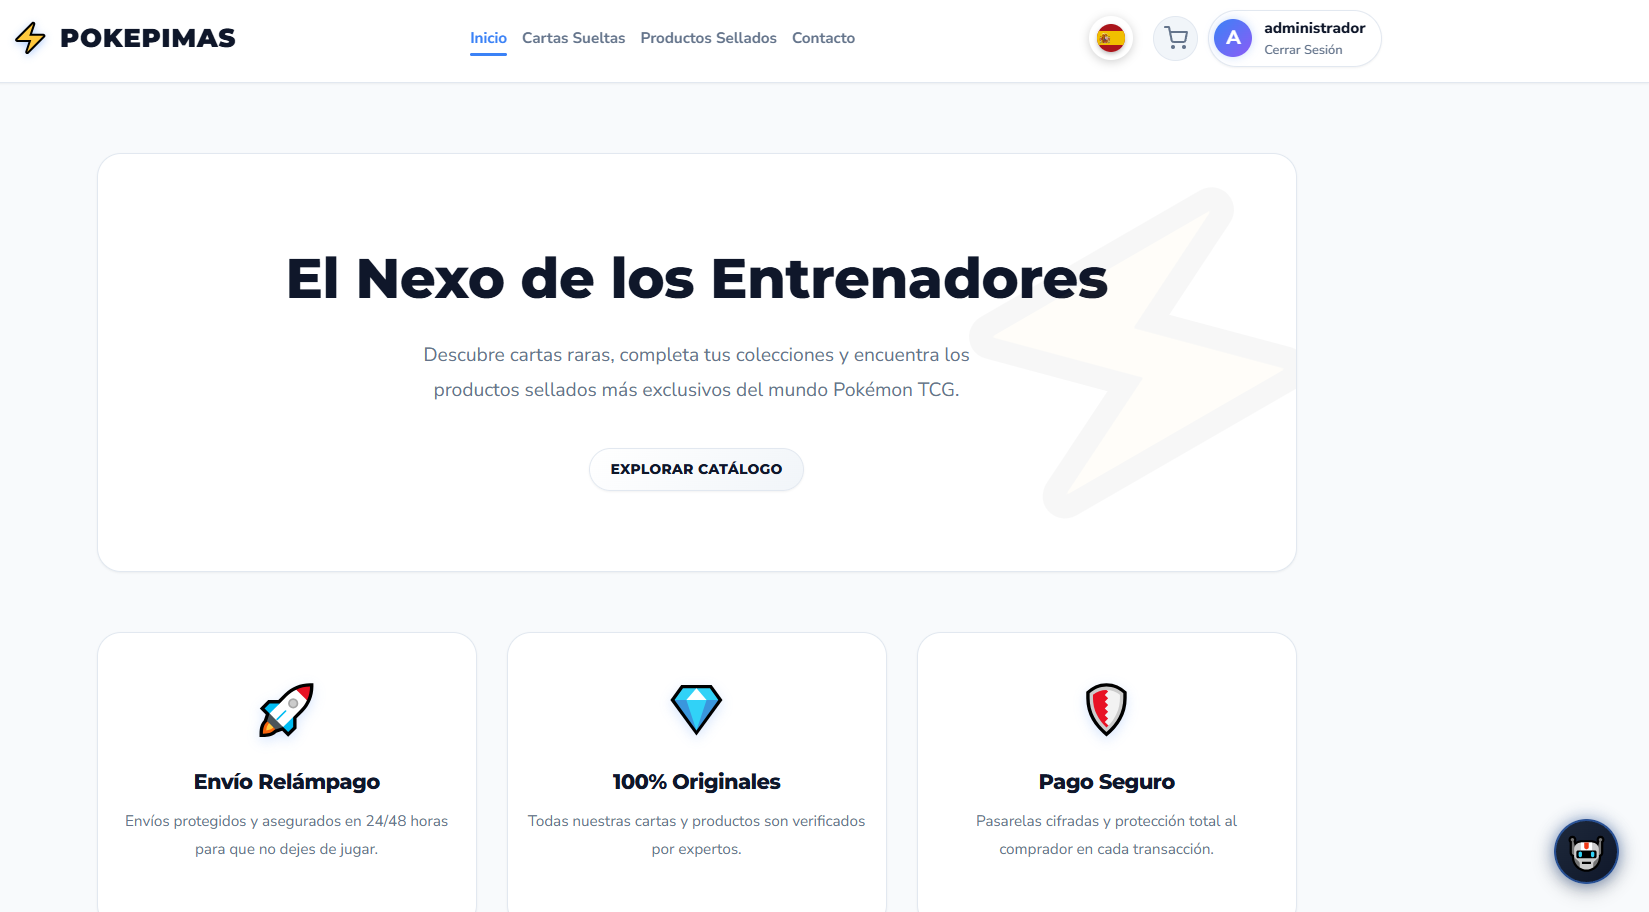
\includegraphics[width=0.8\linewidth]{images/paginaInicio.png}
    \caption{Página de inicio de la tienda web.}
\end{figure}

\begin{figure}[H]
    \centering
    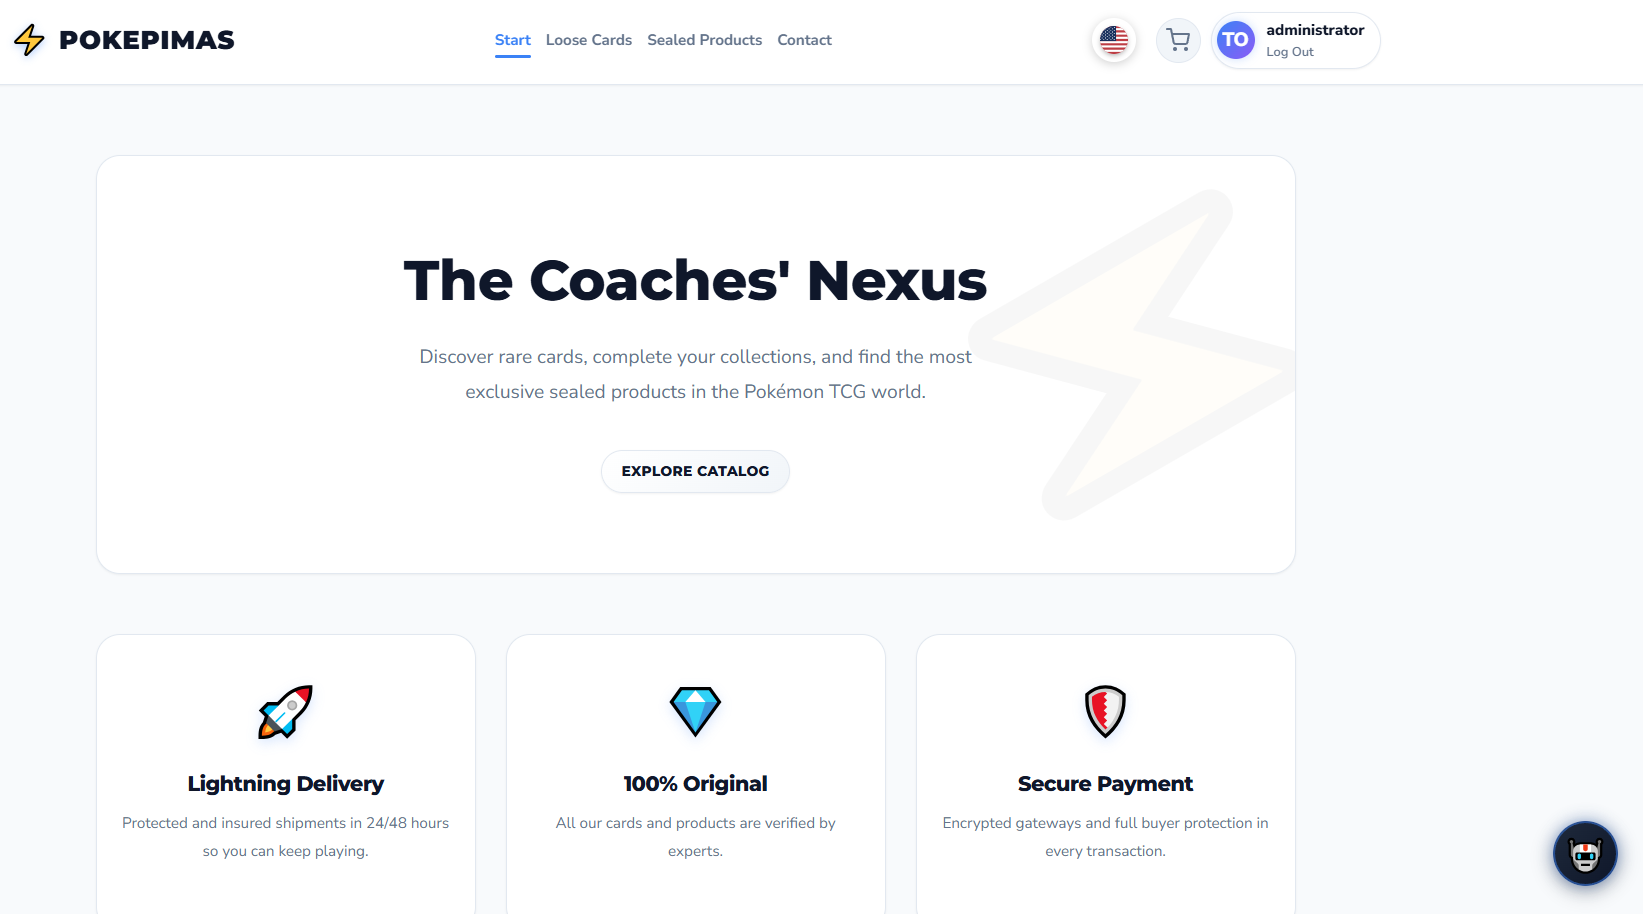
\includegraphics[width=0.8\linewidth]{images/inicioIngles.png}
    \caption{Página de inicio traducida al inglés mediante las banderas.}
\end{figure}

\subsection{Proceso de Compra}
\begin{figure}[H]
    \centering
    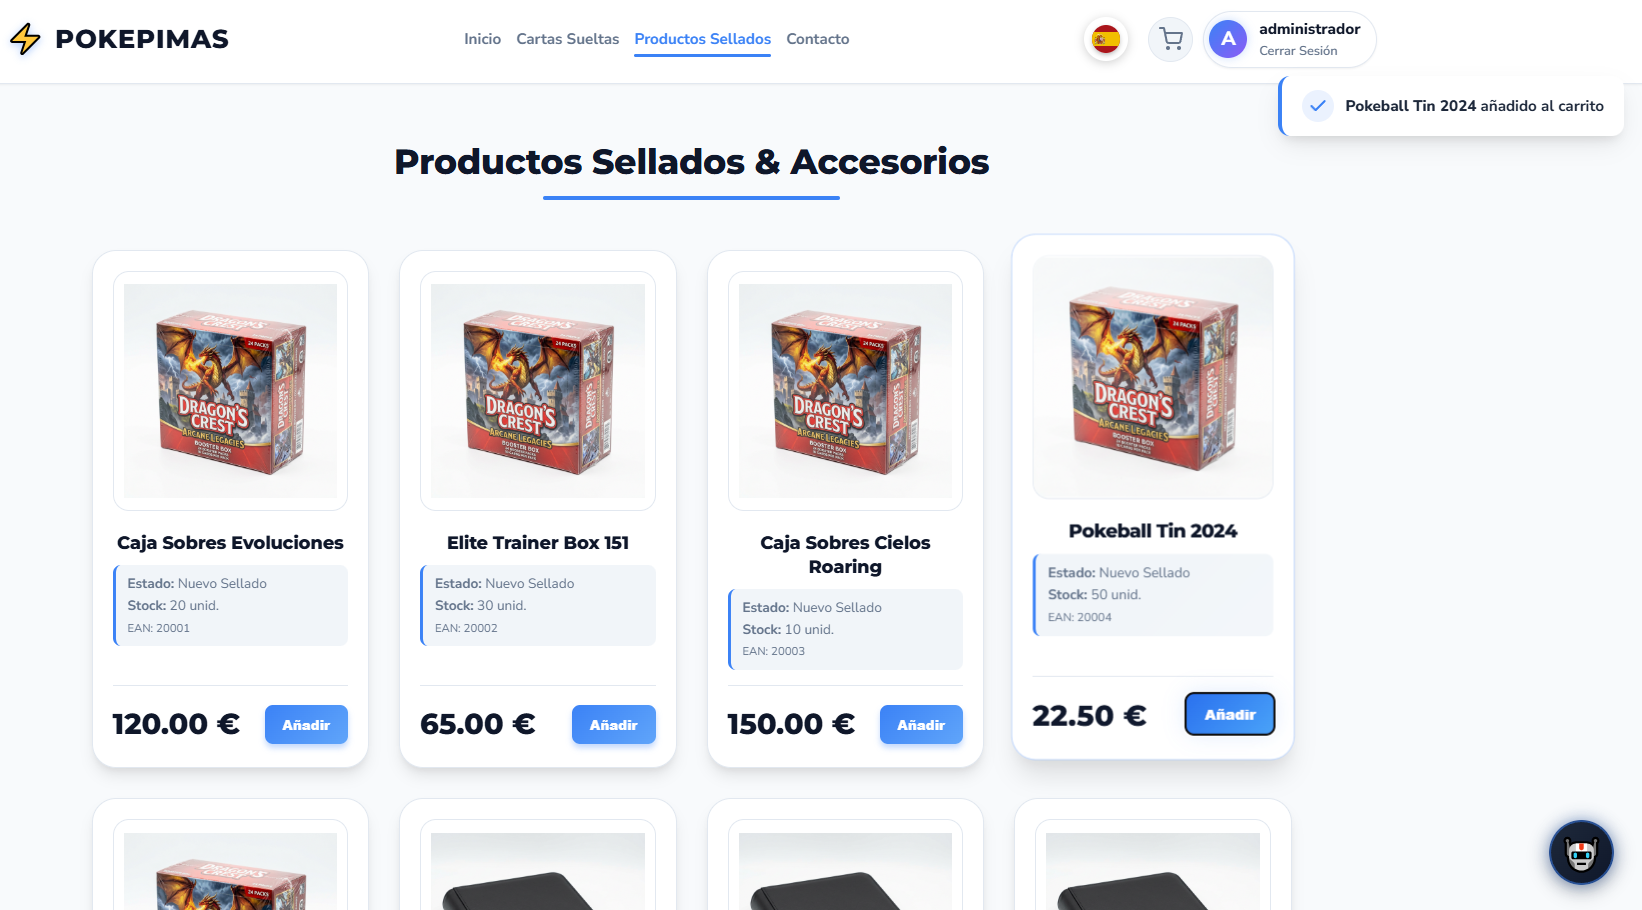
\includegraphics[width=0.8\linewidth]{images/productosSellados+añadirArticulo.png}
    \caption{Vista de productos sellados al añadir un artículo al carrito.}
\end{figure}

\begin{figure}[H]
    \centering
    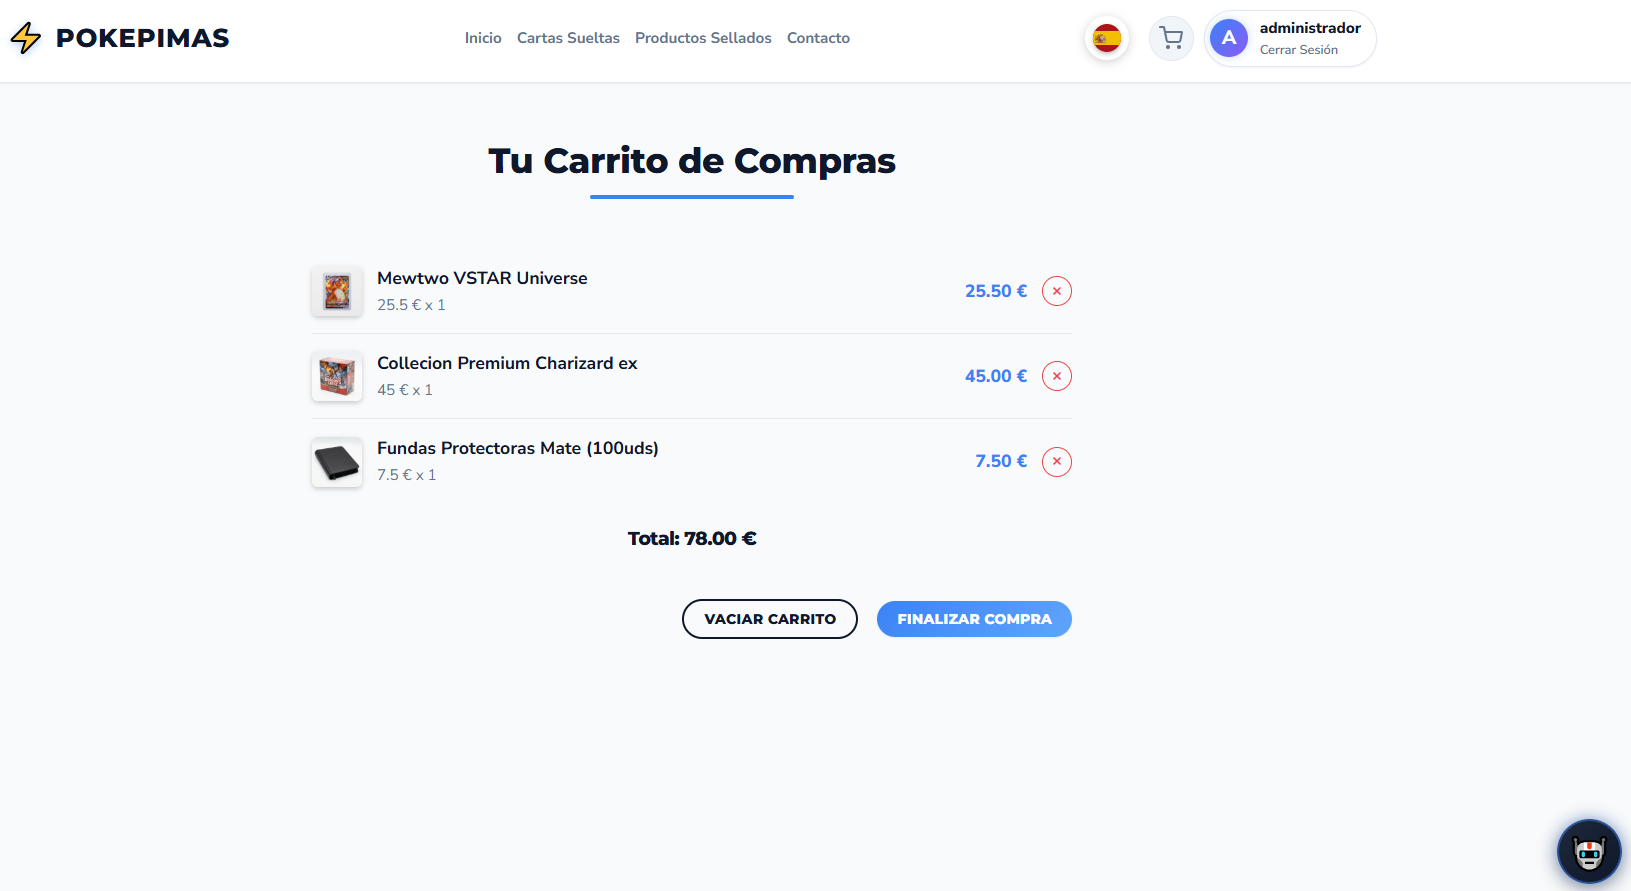
\includegraphics[width=0.8\linewidth]{images/carrito.png}
    \caption{Carrito de compra con los productos añadidos.}
\end{figure}

\subsection{Verificación y Acceso}
\begin{figure}[H]
    \centering
    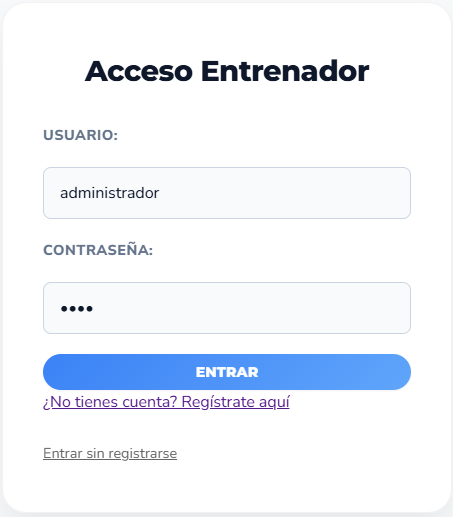
\includegraphics[width=0.8\linewidth]{images/accesoLogin.png}
    \caption{Página de login con un inicio de sesión básico basado en un formulario.}
\end{figure}

\begin{figure}[H]
    \centering
    
\includegraphics[width=0.8\linewidth]{images/correoVerificación.png}
    \caption{Correo con el código de verificación de la cuenta.}
\end{figure}

\begin{figure}[H]
    \centering
    
\includegraphics[width=0.8\linewidth]{images/verificacion.png}
    \caption{Página donde debemos meter el código que nos ha llegado para completar la verificación de la cuenta.}
\end{figure}

\subsection{Herramientas de Inteligencia Artificial}
\begin{figure}[H]
    \centering
    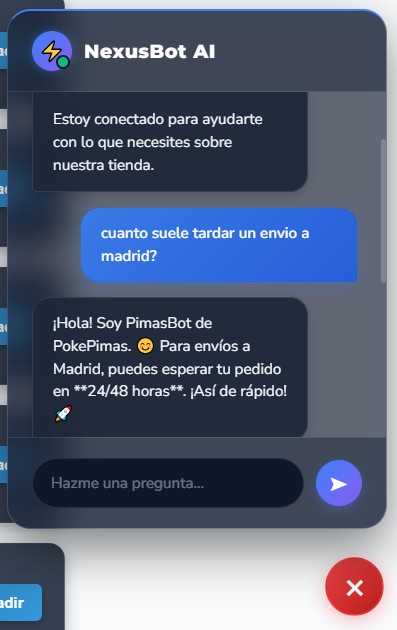
\includegraphics[width=0.8\linewidth]{images/ejemploBot.png}
    \caption{Ejemplo de conversación con el chatbot de la tienda.}
\end{figure}

\begin{figure}[H]
    \centering
    
\includegraphics[width=0.8\linewidth]{images/ejemploBot2.png}
    \caption{El chatbot resolviendo dudas.}
\end{figure}

\begin{figure}[H]
    \centering
    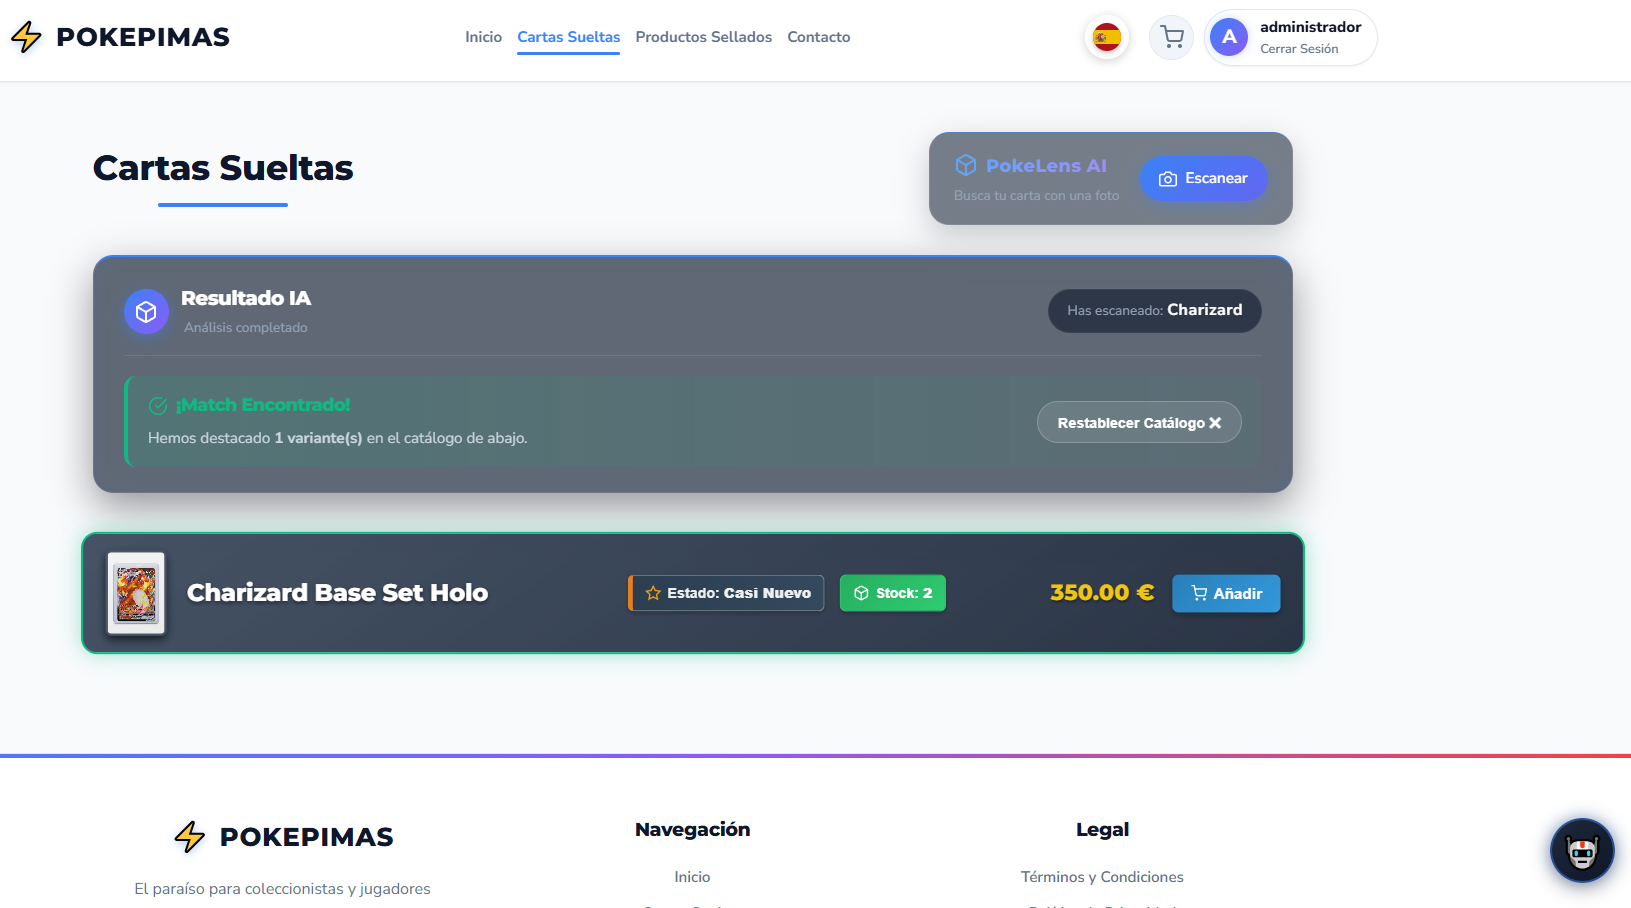
\includegraphics[width=0.8\linewidth]{images/pokeLensWorking.png}
    \caption{Herramienta PokeLens detectando una carta con éxito.}
\end{figure}

\begin{figure}[H]
    \centering
    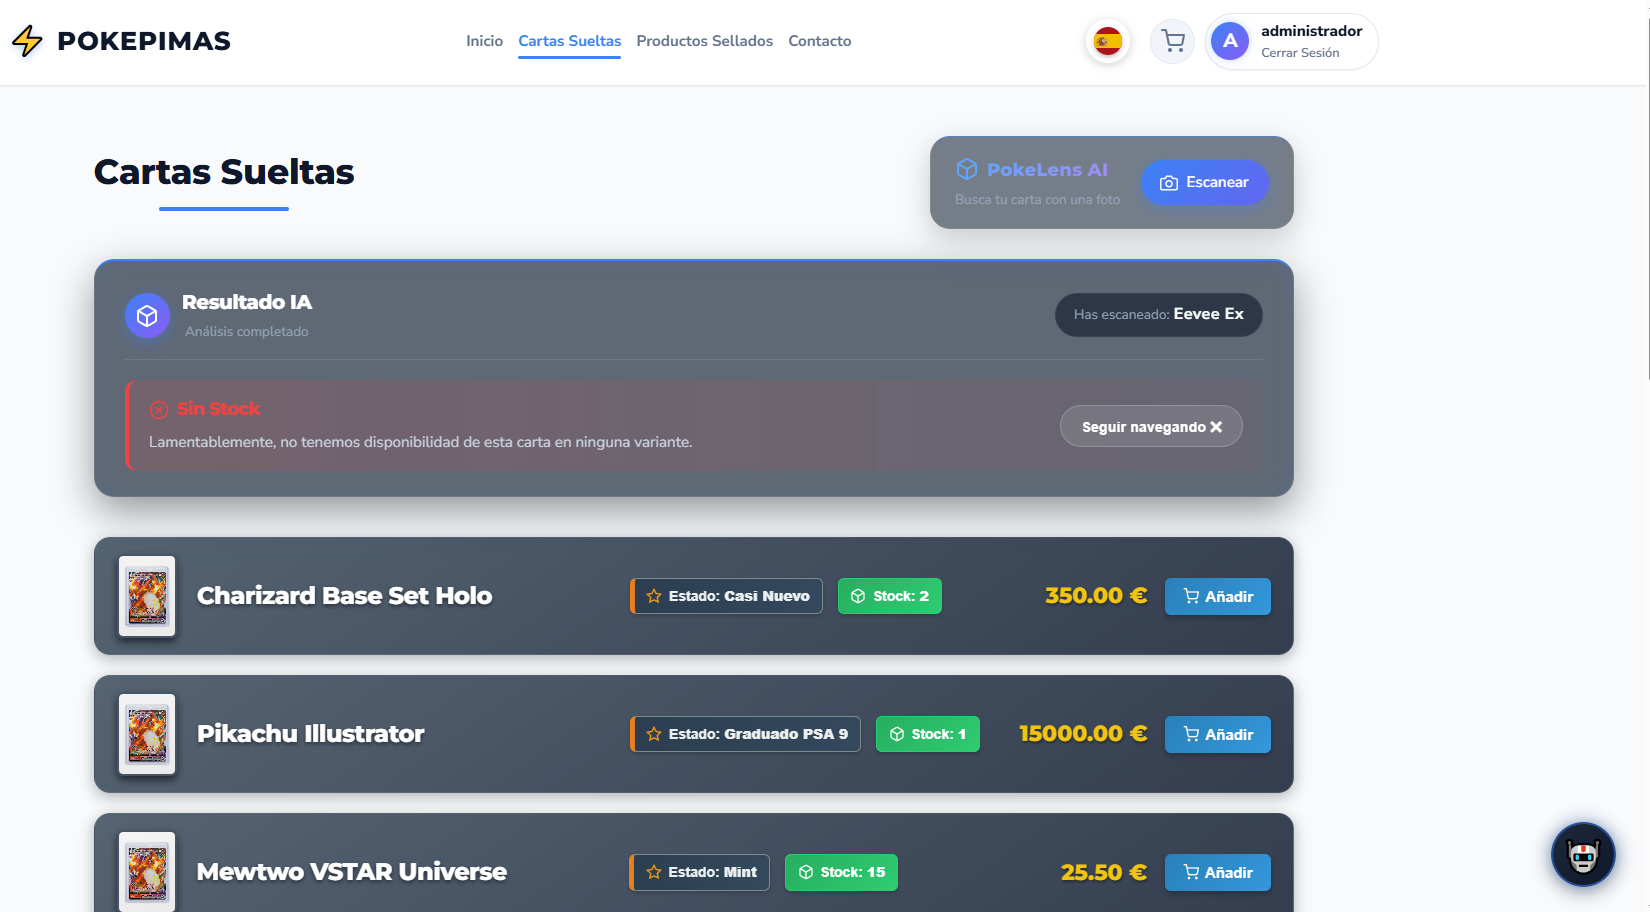
\includegraphics[width=0.8\linewidth]{images/pokeLensNot.png}
    \caption{Herramienta PokeLens cuando no encuentra la carta en la base de datos.}
\end{figure}

\subsection{Atención al Cliente}
\begin{figure}[H]
    \centering
    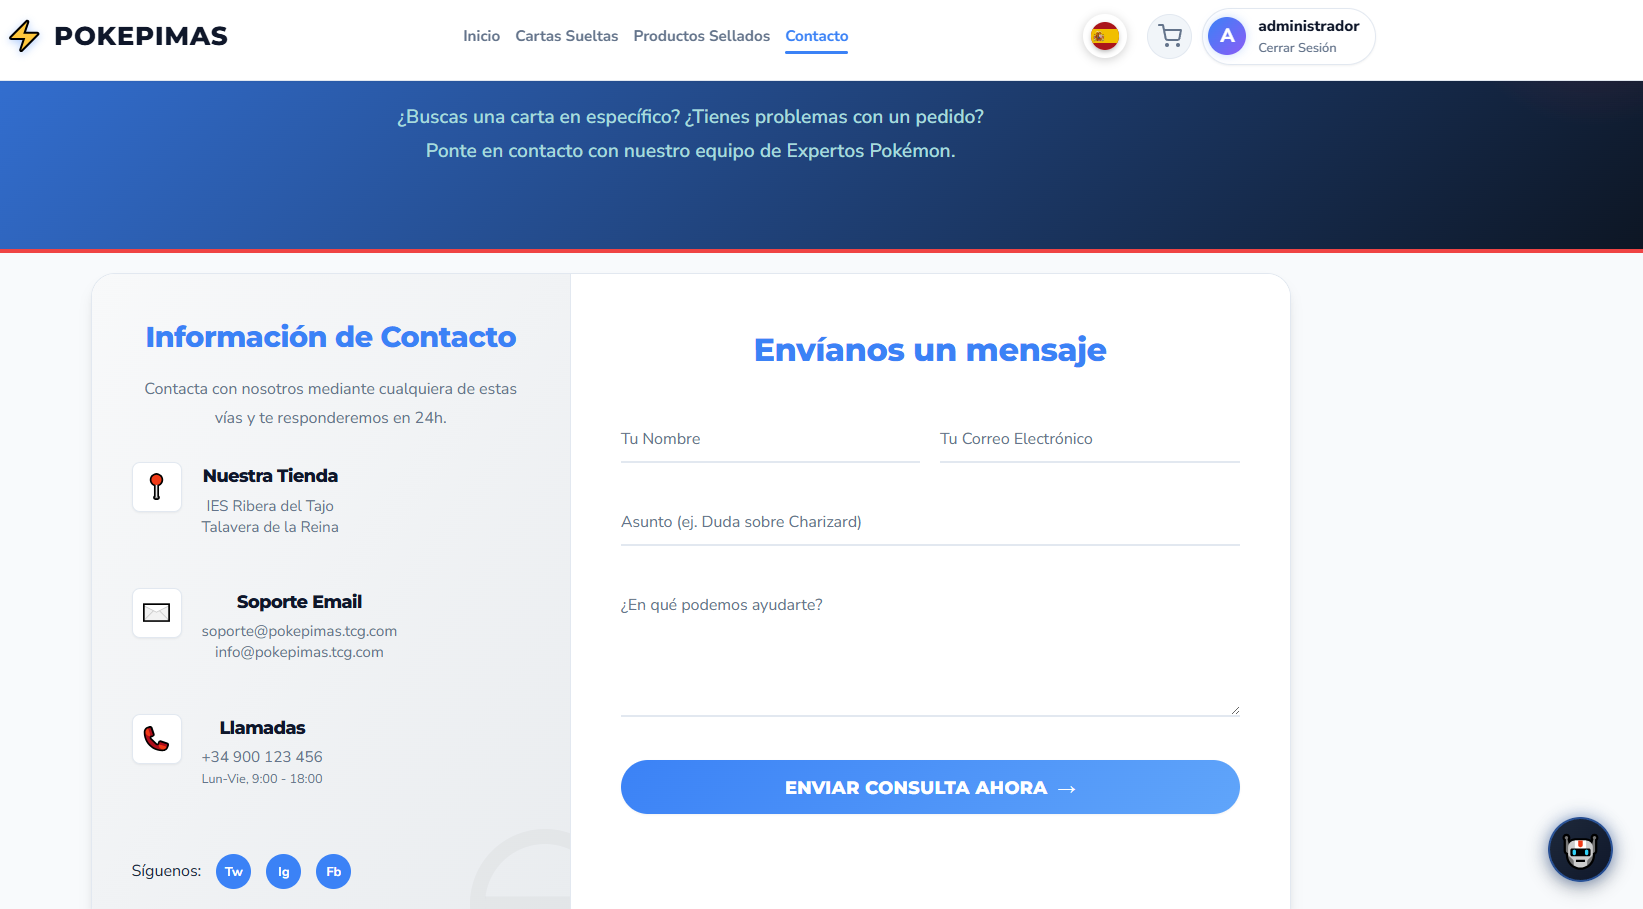
\includegraphics[width=0.8\linewidth]{images/contacto.png}
    \caption{Página de contacto.}
\end{figure}

\subsection{Vista Móvil (Diseño Responsive)}
\begin{figure}[H]
    \centering
    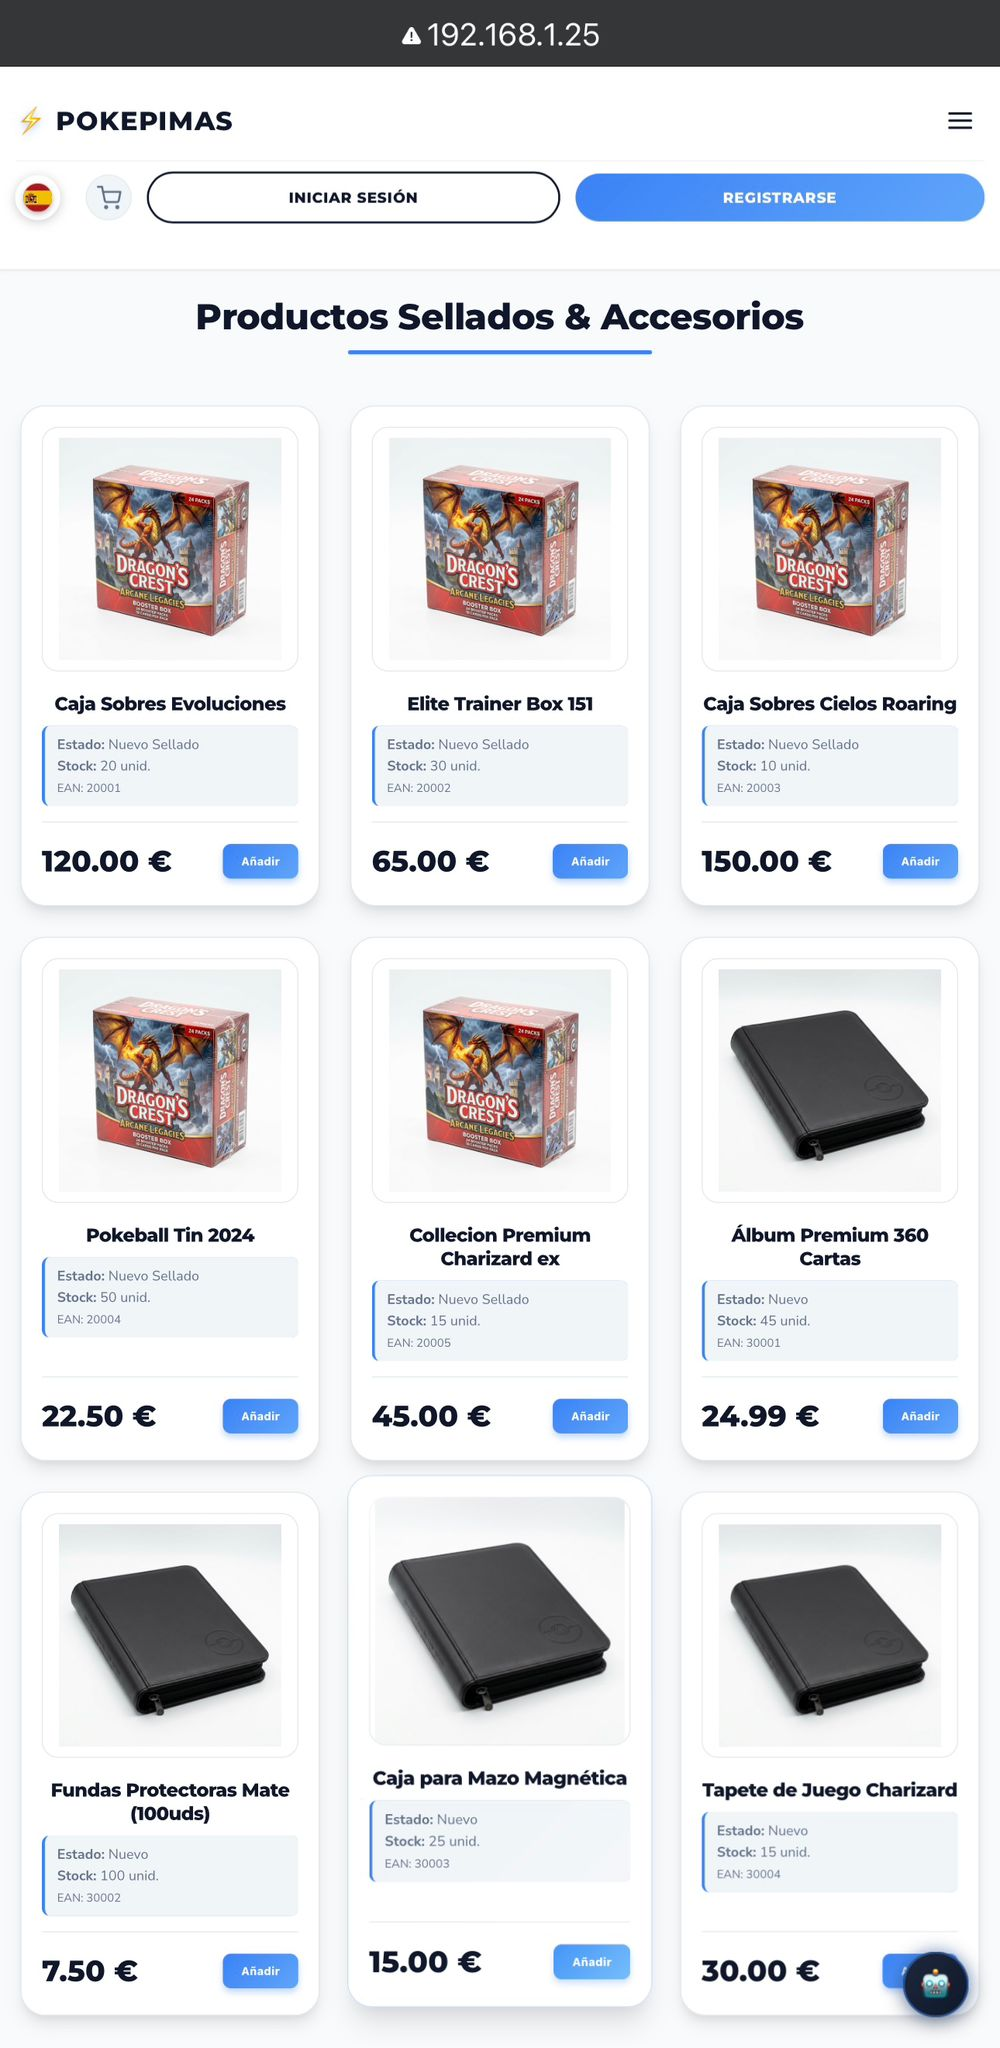
\includegraphics[width=0.45\linewidth]{images/movil1.jpeg}
    \caption{Visualización general de la interfaz adaptada a un teléfono móvil.}
\end{figure}

\begin{figure}[H]
    \centering
    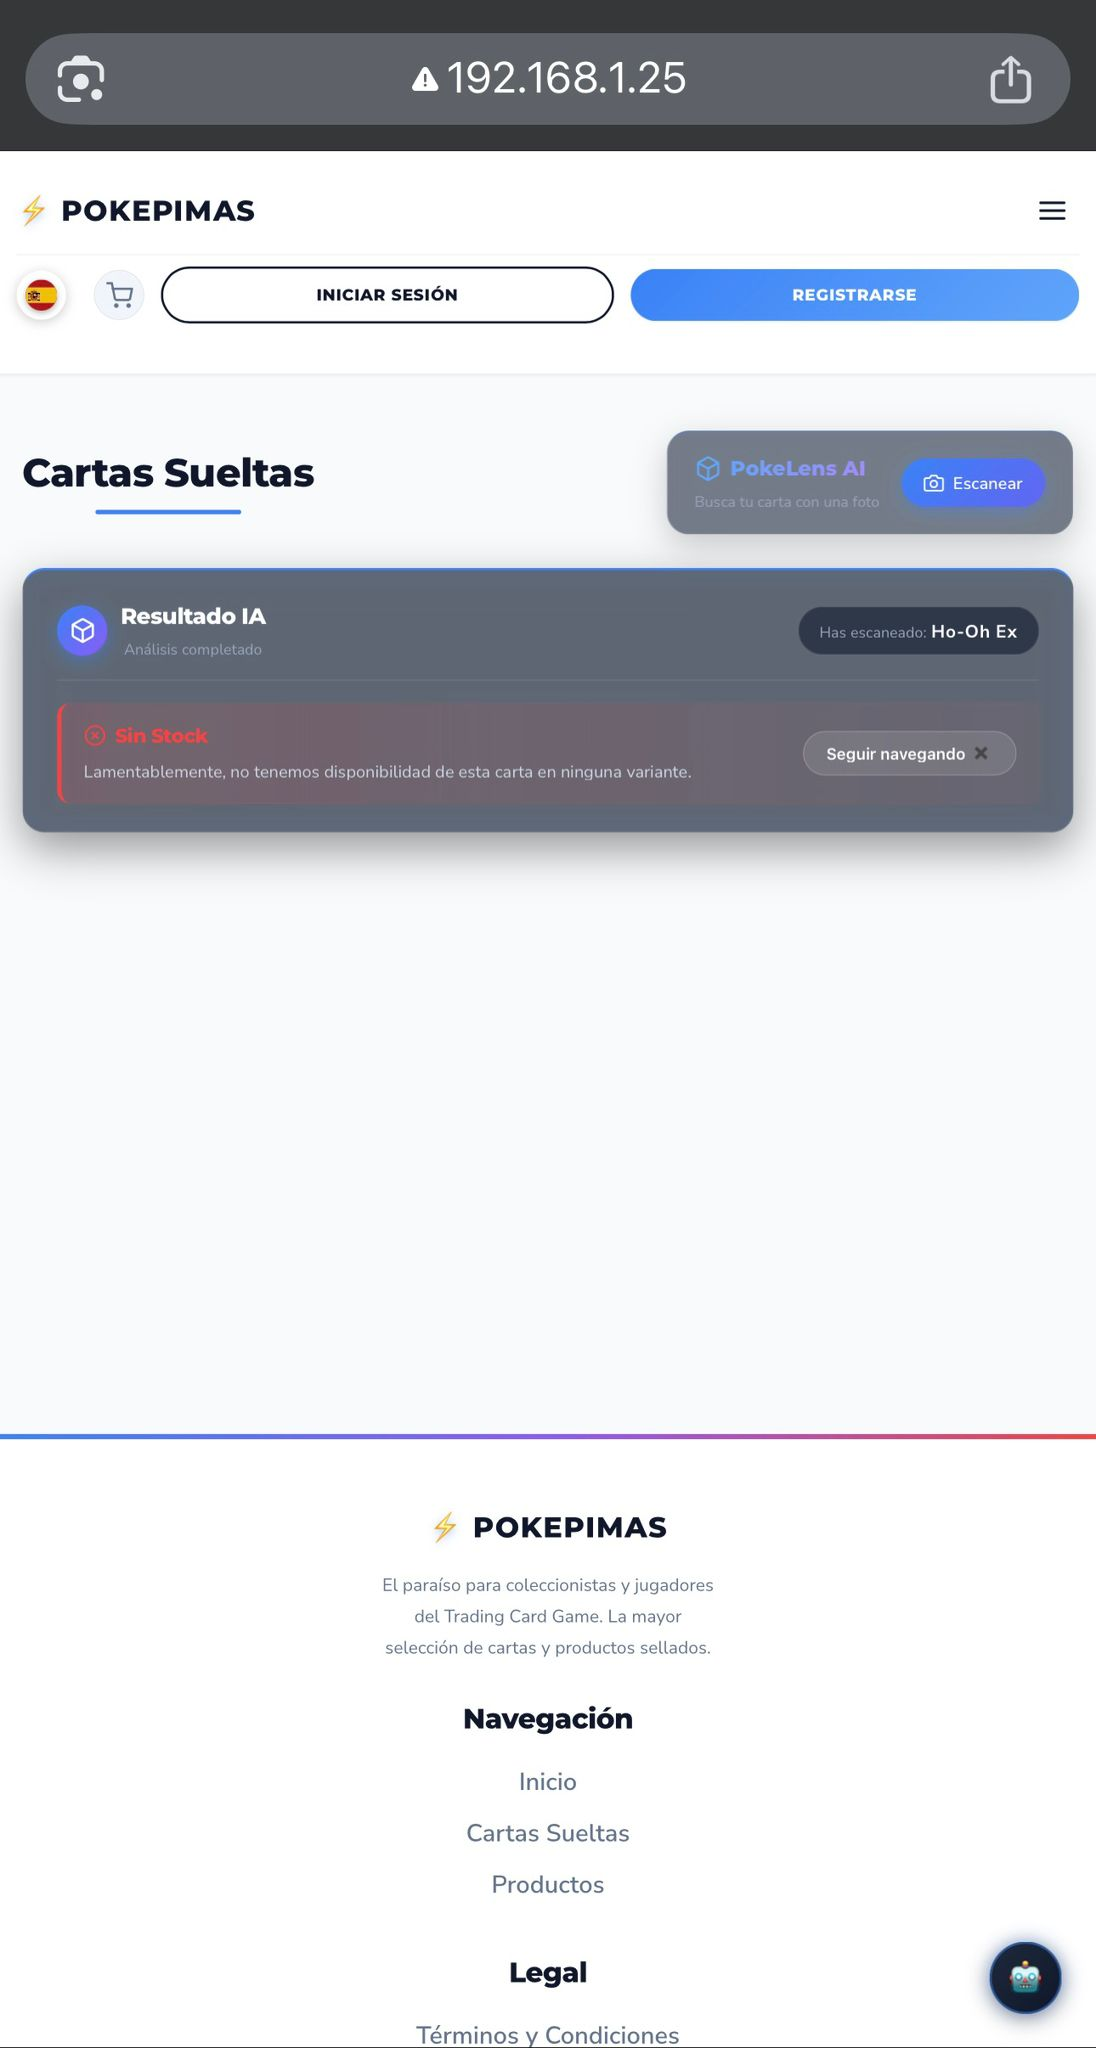
\includegraphics[width=0.45\linewidth]{images/movil2.jpeg}
    \caption{Menú de navegación principal desplegado en formato móvil.}
\end{figure}

\begin{figure}[H]
    \centering
    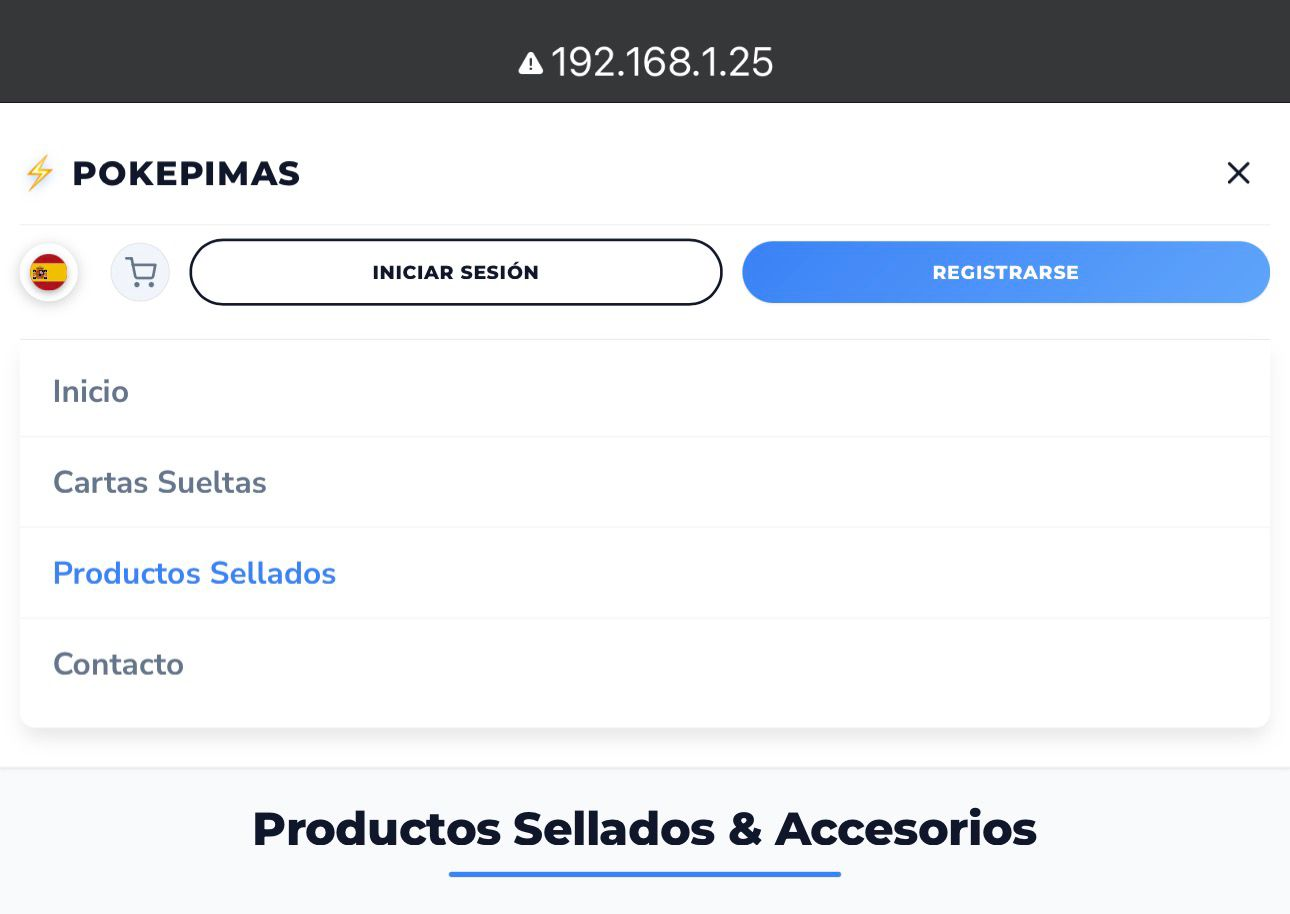
\includegraphics[width=0.45\linewidth]{images/movil3.jpeg}
    \caption{Vista del catálogo de productos y carrito adaptados a la pantalla táctil.}
\end{figure}

\end{document}
